\section{Conference Management}

The Conference Planning Committee is separated into three categories: Co-Chairs, Directors, Coordinators. The three co-chairs are responsible for setting up major milestones and ensuring that those milestones are met. Together they oversee all three subcommittees. They will serve as the primary contacts between subcommittee chairs and the faculty as well as professionals. The co-chairs have the final word on all conference decisions. They serve as the faces of the conference. In this proposal we have decided to add a novel Co-Chair position: Diversity Co-Chair. This addition reflects our goal of celebrating the people behind the science and make this conference experience accessible to as many people as possible. 
The Directors are in charge of specialized subcommittees and are responsible for making decisions in those areas. They must communicate with their subcommittees and with other directors to make sure there are no conflicting decisions. The coordinators work in an even more specialized area and help the directors by handling a single task.\\

% \vspace{1cm}

% ===============================================
% This is the hierarchy breakdown
% ===============================================
% \begin{center}
% 	\begin{tikzpicture}[
% 		chair/.style={rectangle, text centered, draw,fill=blue!20, execute at begin node={\begin{varwidth}{9em}},
%    		execute at end node={\end{varwidth}}},
%    		committee/.style={rectangle,draw,fill=green!40, text centered, execute at begin node={\begin{varwidth}{7em}},
%    		execute at end node={\end{varwidth}}},
%    		coordinator/.style={rectangle,draw,fill=red!30, text centered, execute at begin node={\begin{varwidth}{7em}},
%    		execute at end node={\end{varwidth}}},
% 		grandchild/.style={grow=down,xshift=1em,anchor=west,
% 		edge from parent path={(\tikzparentnode.south) |- (\tikzchildnode.west)}, execute at begin node={\begin{varwidth}{8em}},
%    		execute at end node={\end{varwidth}}},
% 		first/.style={level distance=12ex},
% 		second/.style={level distance=24ex},
% 		third/.style={level distance=36ex},
% 		level 1/.style={sibling distance=11em}]
% 	    % Parents
% 	    \coordinate
% 	      child[grow=left] {node[chair,anchor=east]{General Co-Chair \\ (Sam Dotson)}}
% 	      child[grow=right] {node[chair,anchor=west]{Technical Co-Chair\\ (Jeremy Mettler)}}
% 	      child[grow=down,level distance=3ex]
% 	    [edge from parent fork down]
% 	    % Children and grandchildren
% 	    child{node[committee] {Non-Technical Subcommittee}
% 	      child[grandchild,first] {node[chair]{Logistics Chair}}
% 	      child[grandchild,second] {node[coordinator]{Hotels and Transportation}}
% 	      child[grandchild,third] {node[coordinator] {Hospitality and Catering}}}
% 	    child {node[committee] {Media Subcommittee}
% 	      child[grandchild, first] {node[chair] {Publications Chair}}
% 	      child[grandchild, second] {node[coordinator]{Media}}
% 	      child[grandchild, third] {node[coordinator] {Program}}}
% 	    child{node[committee] {Financial Subcommittee}
% 	      child[grandchild,first] {node[chair]{Financial Chair}}
% 	      child[grandchild,second] {node[coordinator]{Registration}}
% 	      child[grandchild,third] {node[coordinator]{Sponsorship}}}
% 	    child {node[committee]{Technical Subcommittee}
% 	      child[grandchild,first] {node[chair]{Sessions Chair}}
% 	      child[grandchild,second] {node[coordinator]{Workshops}}
% 	      child[grandchild,third] {node[coordinator]{Career Fair}}};
% 	\end{tikzpicture}
% \end{center}
\begin{center}
	\begin{tikzpicture}
		\node (gen chair) [chair] {General Co-Chair (Sam Dotson)};
		\node (tech chair) [chair, right of = gen chair, xshift = 5cm] {Technical Co-Chair (Jeremy Mettler)};
		\node (div chair) [chair, left of = gen chair, xshift = -5cm] {Diversity Co-Chair (Nate Reid)};

		\node (log chair) [director, below of = gen chair, xshift = -3.75cm, yshift = -2cm] {Logistics Chair\\ (Natalie Gaughan)};
		\node (med coord) [coordinator, below of = gen chair, xshift = 0.0cm, yshift = -3cm] {Media Coordinator (Nathan Ryan)};
		\node (prog coord) [coordinator, below of = log chair, yshift = -2cm] {Program Coordinator (Dilan K.)};
		\node (hat coord) [coordinator, below of = prog coord, yshift = -2cm] {Hotels and Transport (Gavin Davis)};
		\node (hoa coord) [coordinator, below of = hat coord, yshift = -2cm] {Hospitality and Accomodations\\ (Brady Moran)};
		\node (tours coord) [coordinator, below of = hoa coord, yshift = -2cm] {Tours Coordinator (Anna Balla)};


		\node (tsc chair) [director, below of = tech chair, xshift = 2cm, yshift = -2cm] {Technical Sub-Committee Chair (Gwendolyn Chee)};
		\node (work coord) [coordinator, below of = tsc chair, yshift = -2cm] {Workshops Coordinator\\(Roberto Fairhurst)};
		\node (sesh coord) [coordinator, below of = work coord, yshift = -2cm] {Sessions Coordinator (Zach Jeckell)};
		\node (cf coord) [coordinator, below of = sesh coord, yshift = -2cm] {Career Fair Coordinator (Greg Golba)};
		
		\node (fin chair) [director, below of = tech chair, xshift = -2.25cm, yshift = -2cm] {Financial Chair\\(Jack Stahl)};
		\node (spon coord) [coordinator, below of = fin chair, yshift = -2cm] {Sponsorships Coordinator (Jimmy Shehee)};
		\node (reg coord) [coordinator, below of = spon coord, yshift = -2cm] {Registration Coordinator\\(Jasmine Dinari)};

		\draw  (gen chair) -- (tech chair);
		\draw  (gen chair) -- (div chair);
		\draw  (gen chair) -- (log chair);
		\draw  (log chair) -- (prog coord);
		\draw  (prog coord) -- (hat coord);
		\draw  (hat coord) -- (hoa coord);
		\draw  (hoa coord) -- (tours coord);
		\draw  (gen chair) -- (med coord);
		\draw  (tech chair) -- (fin chair);
		\draw  (gen chair) -- (fin chair);
		\draw  (tech chair) -- (tsc chair);
		\draw  (fin chair) -- (spon coord);
		\draw  (spon coord) -- (reg coord);
		\draw  (tsc chair) -- (work coord);
		\draw  (work coord) -- (sesh coord);
		\draw  (sesh coord) -- (cf coord);
		\draw  (div chair) -- (log chair);

	\end{tikzpicture}
\end{center}

% ===============================================
% ===============================================
% ===============================================




\newpage
\subsection{Position Responsibilities}

\begin{itemize}
	\item $\large\textbf{\textit{General Co-Chair}}$\\
	In addition to the responsibilities outlined above, the General Co-Chair oversees the
	Non-technical Subcommittee, the Media Coordinator, and the Financial Subcommittee. He works with the Technical Co-Chair in talking to sponsors, companies, and planning full committee meetings. 
	\item $\large\textbf{\textit{Technical Co-Chair}}$\\
	In addition to the responsibilities outlined above, the Technical Co-Chair primarily oversees the
	Technical Subcommittee. Works with the General Co-Chair to plan full committee meetings and completes any remaining tasks to ensure that milestones are met.
	\item $\large\textbf{\textit{Diversity Co-Chair}}$\\
	In addition to the responsibilities outlined above, the Diversity 
                Co-Chair is responsible for making sure the conference is as 
                inclusive, diverse, and accessible as possible. This includes: 
                contacting minority serving institutions to encourage their 
                students to attend the conference, ensuring socials and dinners 
                are accessible, verifying that the final list of speakers has 
                adequate representation, engaging with the national Diversity and 
                Inclusion in ANS Committee, and more. We believe the example set 
                by UIUC will make this role a staple of future conferences. 

	\item $\textbf{Non-Technical Subcommittee}$\\
	The Non-Technical Subcommittee oversees, arranges, and executes all actions related to hospitality, transportation, special events, and non-technical workshops and panels. This committee keeps the theme of the conference in mind when organizing all events. They ensure that the conference runs smoothly.
	\begin{itemize}
		\item[$\circ$] $\textbf{Logistics Chair}$\\
		The Logistics Chair is in charge of planning all tours and non-technical workshops and panels. Organizes speakers during dinners. Recruits student volunteers to staff events and sessions during the conference.
		Also responsible for keeping track of the subcommittee and reporting to the Co-Chairs.
		\item[$\circ$] $\textbf{Hotels and Transportation Coordinator}$\\
		Coordinates with ANS National to negotiate room rates and room blocks for hotels. Reserves buses for the 
		necessary times and events. Works with the Hospitality and Catering Coordinator and the Logistics Chair.
		\item[$\circ$] $\textbf{Hospitality and Catering Coordinator}$\\
		Responsible for planning and organizing all catered meals for 
                        the conference. That includes contacting the catering services, reserving the venues where meals are held, and making sure the venues are staffed.
		\item[$\circ$]$\textbf{Tours Coordinator}$\\
		The tours coordinator organizes tours and works with the transportation coordinator to ensure that transportation is available during the conference for these tours.
		\item[$\circ$]$\textbf{Program Coordinator}$\\
		The program coordinator creates programs for the conference, sets the conference schedule to minimize overlap between events and increase student involvement. Communicates with other coordinators and subcommittees about the schedule of events. Designs and purchases T-shirts for attendees. Arranges gift bags for attendees. Works with sponsorship coordinator to create gift bags.
	\end{itemize}
	\item $\textbf{Financial Subcommittee}$\\
	The Financial Subcommittee oversees, arranges, and executes all actions related to banking, sponsorship, registration, reimbursement, budgeting, and monetary exchanges. This committee works closely with the General and Technical Co-Chairs.
	\begin{itemize}
		\item[$\circ$] $\textbf{Financial Chair}$\\
		Manages the ANS Planning Committee account with Busey Bank and ANS National. The account coordinator is also responsible for keeping track of receipts, setting a budget for the committee, keeps track of all transactions, 
		\item[$\circ$] $\textbf{Registration Coordinator }$
		Handles the registration for professional and student attendees. Communicates the number of attendees to the Program Coordinator. 
		\item[$\circ$] $\textbf{Sponsorship Coordinator}$\\
		Assists the Financial Co-Chair with matters involving sponsorship as well as working closely with the Registration and Account Coordinators and the General and Technical Co-Chairs. Works with the Program Coordinator on gift bag items and works with the Career Fair Coordinator.
	\end{itemize}
	\item $\textbf{Technical Subcommittee}$\\
	The Technical Subcommittee works with the Technical Co-Chair to process student abstracts and set up 
	technical workshops, panels and sessions. 
	\begin{itemize}
		\item[$\circ$] $\textbf{Technical Subcommittee Chair}$\\
		 Also responsible for ensuring that judges understand the judging criteria, and organizes the award ceremony.
		Keeps track of subcommittee progress and reports to the General and Technical Co-chairs.
		\item[$\circ$] $\textbf{Sessions Coordinator}$\\
		Responsible for organizing presentation, poster sessions, and technical
		panels. Makes sure that all rooms are properly set up with equipment to ensure smooth technical sessions.
		\item[$\circ$] $\textbf{Workshops Coordinator}$\\
		Organizes workshops locations, times, staffing, costs, supplies, student enrollment
		and any other tasks required to have successful workshops. Also assists the Sessions Chair when needed.
		\item[$\circ$] $\textbf{Career Fair Coordinator}$\\
		Oversees staffing and support for the career fair as well as working with the Sponsorship
		Coordinator to ensure a successful career fair. Also assists the Sessions Chair when needed.
	\end{itemize}
	\item $\textbf{Media Coordinator}$\\
		The Media Coordinator is responsible for designing the conference website, constantly updating social media presence,
		and obtains information from other members of the planning committee for the website.
\end{itemize}

\newpage
\subsection{Planning Committee Biographies}

\begin{minipage}{0.25\textwidth}
	\centering
	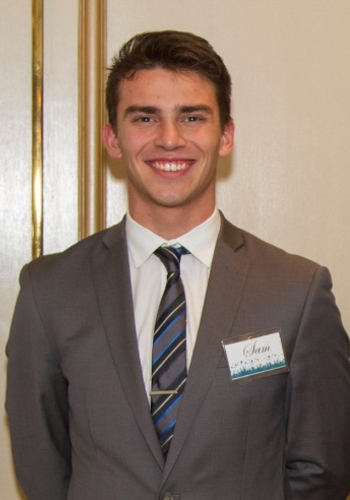
\includegraphics[width=\textwidth]{fmt-dotson.jpg}
\end{minipage}
\begin{minipage}{0.73\textwidth}
	$\textbf{General Co-Chair - Sam Dotson}$\\
Sam graduated with a B.S. in Physics from UIUC in 2019. He attended his first ANS student conference in April 2019 and was so inspired by his experience that he decided to pursue graduate work in nuclear engineering rather than physics. Now he does research on machine learning applications and computational reactor physics with Dr. Kathryn Huff in the ARFC group. Hosting a student conference that will inspire others the way he was inspired is one of his top priorities this year. He has experience planning activities for student organizations such as Guidance for Physics Students (GPS) and has experience fundraising for the College of Lake County (CLC). He helped set a record amount of donations at the 2016 CLC Foundation Gala, where he was an invited speaker and volunteer. He will be attending the ANS National conference in November 2019, as well as the ANS Student Conference 2020 at North Carolina State University.
\end{minipage}

\begin{minipage}{0.25\textwidth}
	\centering
	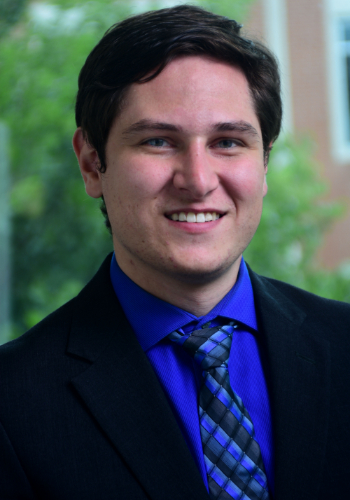
\includegraphics[width=\textwidth]{fmt-mettler.jpg}
\end{minipage}
\begin{minipage}{0.73\textwidth}
	$\textbf{Technical Co-Chair - Jeremy Mettler}$\\
Jeremy graduated with a B.S. in Nuclear, Plasma, and Radiological Engineering from UIUC in 2018, and is now attending as a 2nd-year graduate student studying plasma science under Dr. David Ruzic. He has been heavily involved in the UIUC student chapter of ANS since his freshman year, serving on the executive board for three years as External Vice President and President. Jeremy has attended the past five ANS Student Conferences, which serve as an inspiration for his involvement in this proposal process. He is dedicated to making sure that future generations of students are able to have the same amazing experiences through ANS as he had, especially at the ANS Student Conference. Outside of ANS, he has held a summer internship at Oak Ridge National Lab, and is currently focusing his research towards combined laser-plasma systems for materials processing.
\end{minipage}

\begin{minipage}{0.25\textwidth}
	\centering
	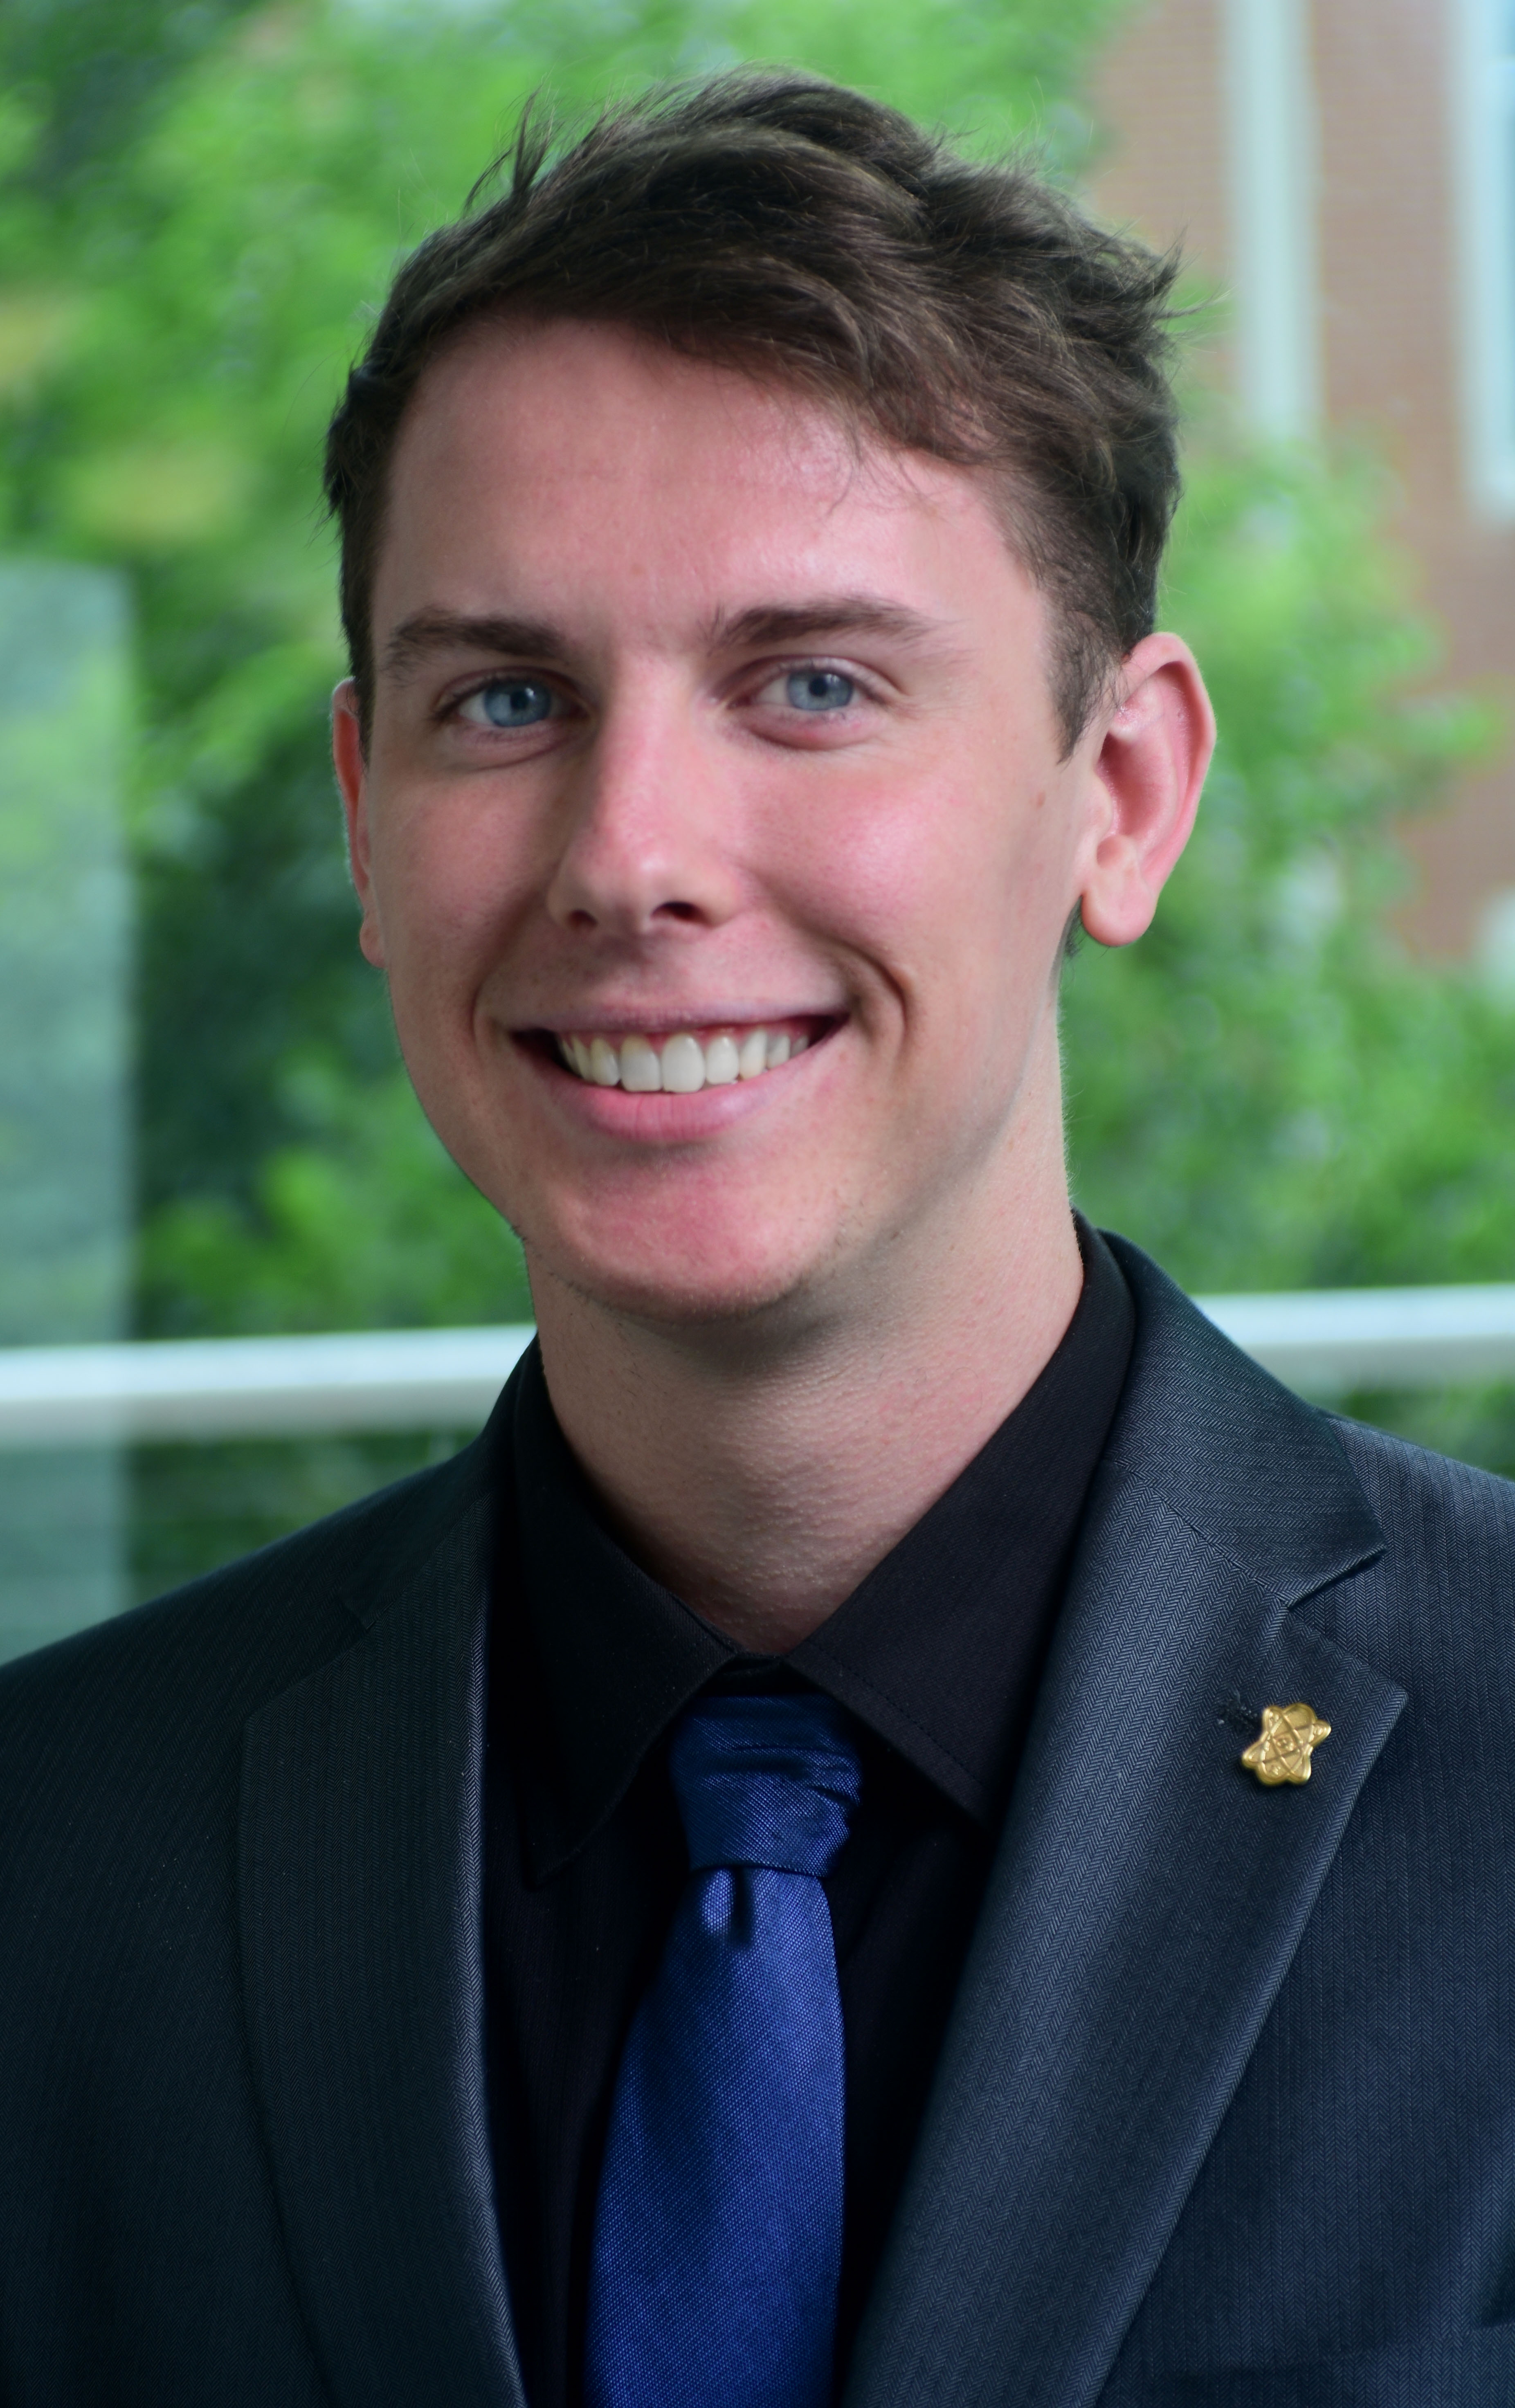
\includegraphics[width=\textwidth]{ncreid2.jpg}
\end{minipage}
\begin{minipage}{0.73\textwidth}
$\textbf{Diversity Co-Chair - Nathan Reid}$\\
	Nate graduated with a B.S. in Nuclear, Plasma, and Radiological Engineering from UIUC in 2016. He is a 4th-year Ph.D. student in the field of fusion and plasma science and engineering under Prof. Jean Paul Allain. Nate is currently conducting his thesis research at Oak Ridge National Laboratory, where he has spent the last three summers working in the nuclear structural materials group under the mentorship of Dr. Lauren Garrison. He will return the UIUC in December 2019. Nate has attended four of the last five ANS Student Conferences and was a student paper competition finalist at the TOFE embedded topical of the 2018 ANS Winter Meeting. Nate has been recognized by the ANS-UIUC for his outstanding graduate service in the last year, and served as the Women in Nuclear UIUC chapter Vice President. He was part of the executive team that received the national student chapter excellence award at the 2019 Women in Nuclear national conference, of which he was awarded a student sponsorship to attend. Nate is ecstatic about working alongside his ANS student section as Diversity Co-Chair and setting goals to bring inclusion to the conference.
\end{minipage}

\begin{minipage}{0.25\textwidth}
	\centering
	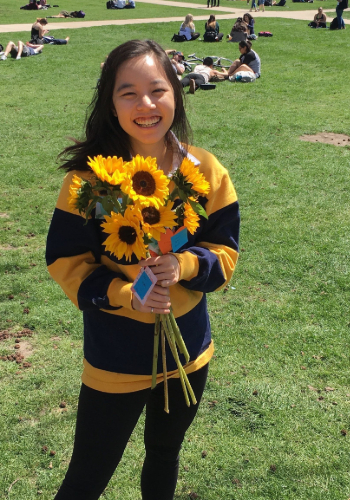
\includegraphics[width=\textwidth]{fmt-chee.jpg}
\end{minipage}
\begin{minipage}{0.73\textwidth}
$\textbf{Technical Subcommittee Chair - Gwendolyn Chee}$\\
	Gwen is a third year graduate student studying fuel cycles for advanced reactor designs with Dr. Kathryn Huff in the ARFC group. Last summer she had an internship at Argonne National Laboratory where she worked on sensitivity analysis of the nuclear fuel complex. She also serves as the president of the UIUC chapter of Women In Nuclear (WIN). Under her leadership, WIN-UIUC was honored with the Best Student Chapter award at the WIN National Meeting in 2019. She has also been involved with ANS and attended the 2018 ANS Student Conference in Florida and will be attending the upcoming ANS Student Conference at NC State in 2020.
\end{minipage}

\begin{minipage}{0.25\textwidth}
	\centering
	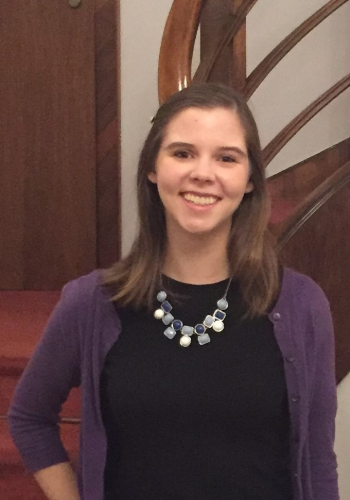
\includegraphics[width=\textwidth]{fmt-gaughan.JPG}
\end{minipage}
\begin{minipage}{0.73\textwidth}
$\textbf{Logistics Chair - Natalie Gaughan}$\\
	Natalie earned her B.S. in Nuclear Engineering from the University of Wisconsin-Madison in 2017. She has completed two summer internships at Argonne National Laboratory where she worked with various neutronics codes. Natalie then spent a year in Vienna as an intern at the International Atomic Energy Agency, where she helped organize and evaluate nuclear data for medical isotope production. She is now a graduate student at UIUC intending to research radiological science and nuclear medicine. As an undergraduate, Natalie attended two ANS student conferences which played a huge role in obtaining internships and inspired her decision to attend graduate school. Natalie knows firsthand how the ANS student conferences can be influential in students’ education and career development, and would love to help younger students experience the same benefits. She will also be attending the upcoming ANS student conference in 2020 at NC State.
\end{minipage}

\begin{minipage}{0.25\textwidth}
	\centering
	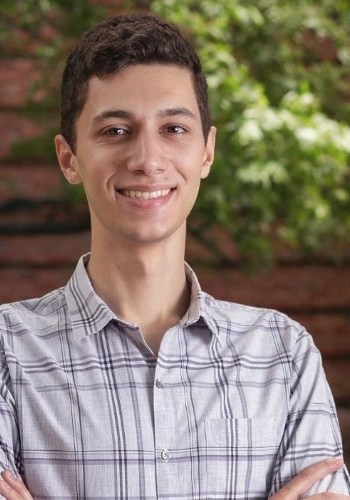
\includegraphics[width=\textwidth]{fmt-stahl.jpg}
\end{minipage}
\begin{minipage}{0.73\textwidth}
	$\textbf{Financial Chair - Jack Stahl}$\\
Jack graduated with a B.S. in Nuclear, Plasma, and Radiological Engineering from UIUC in 2019, and is now a first-year graduate student studying plasma engineering under Dr. David Ruzic. He has been involved in the UIUC student chapter of ANS since his sophomore year and has attended two student conferences. Previously, Jack has spent a summer as an intern at ASML. Jack hopes to help host a student conference that will bolster younger student involvement in ANS.
\end{minipage}

% \vspace{1cm}
\clearpage
\textbf{Financial Subcommittee}\\

\begin{minipage}{0.25\textwidth}
	\centering
	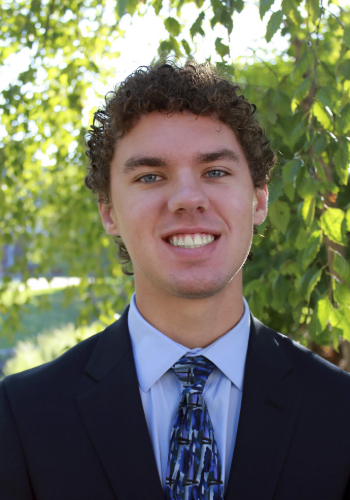
\includegraphics[width=\textwidth]{fmt-shehee.jpg}
\end{minipage}
\begin{minipage}{0.73\textwidth}
	$\textbf{Sponsorship Coordinator - James Shehee}$\\
Jimmy is a junior undergraduate student in UIUC's Nuclear, Plasma, and Radiological Engineering department, with a concentration in power, safety, and the environment. Jimmy has been an active member of the University's ANS student chapter since his freshman year, has held the positions of Secretary and External Vice President, and was chosen to receive the chapter's Undergraduate Outstanding Service Award in the spring of 2019. Jimmy was first introduced to the nuclear industry through the Nuclear Science Merit Badge in Boy Scouts, and he is excited about any opportunity to create similar experiences for students and the public. Outside of ANS, Jimmy is also the President of the Illini Venturing Crew. In the summer of 2019, Jimmy interned at Exelon's Quad Cities Generating Station, and will be returning for another summer in 2020. He is excited to attend his first ANS Student Conference in March 2020 at North Carolina State University.
\end{minipage}

\begin{minipage}{0.25\textwidth}
	\centering
	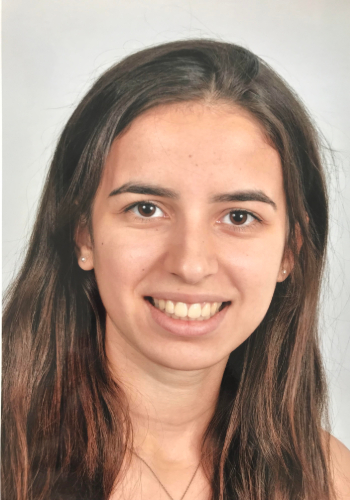
\includegraphics[width=\textwidth]{fmt-dinari.jpg}
\end{minipage}
\begin{minipage}{0.73\textwidth}
	$\textbf{Registration Coordinator - Jasmine Dinari}$\\
Jasmine is a freshman studying Nuclear, Plasma, and Radiological Engineering at UIUC, as well as minors in French and Physics. She is starting research with Dr. Andruczyk, who is currently at the head of the HIDRA project. Powering the world through nuclear is one of her main interests, and she later hopes to participate in nuclear fusion research. The ANS Student Conference is an  amazing opportunity to share her interests in nuclear science. She gained organizational and leadership experience through various extracurriculars in high school and currently serves as the Professional Development Chair for the UIUC student chapter of Women in Nuclear. She plans on attending the 2020 ANS Student Conference at NC State.
\end{minipage}

\vspace{1cm}
\textbf{Technical Subcommittee}\\

\begin{minipage}{0.25\textwidth}
	\centering
	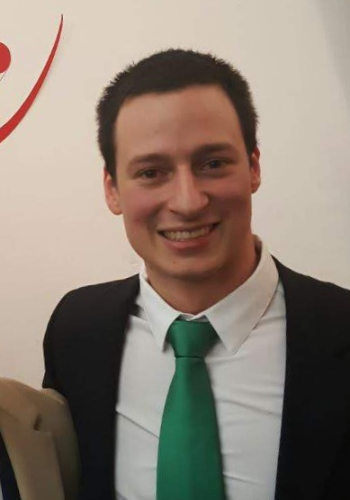
\includegraphics[width=\textwidth]{fmt-fairhurst.jpg}
\end{minipage}
\begin{minipage}{0.73\textwidth}
	$\textbf{Workshops Coordinator - Roberto Fairhurst}$\\
Roberto graduated with a B.S. in Nuclear Engineering from Instituto Balseiro (Argentina) April 2018. He is now a 2nd-year graduate student at UIUC. He does research on computational multi-physics solvers applied to advanced reactors as part of the Advanced Reactors and Fuel Cycle group under the supervision of Dr. Kathryn Huff. He got experience in the organization of conferences during the planning and development of a technical workshop (TWOFCS19) that took place at UIUC in June 2019. His motivation for hosting a student conference is his passion for Nuclear Energy and his desire to transmit this passion to other students. He believes hosting the student conference at UIUC will help the field grow and thrive. This is also an opportunity to meet other people working in the field, share life experiences, and develop a stronger network.
\end{minipage}

\begin{minipage}{0.25\textwidth}
	\centering
	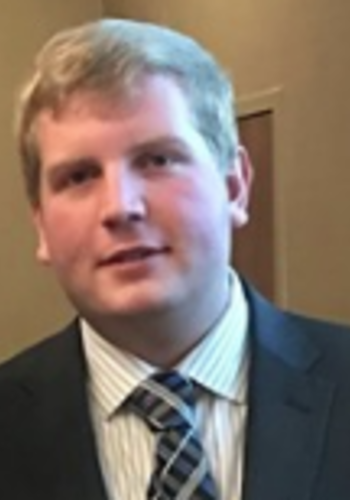
\includegraphics[width=\textwidth]{fmt-jeckell.png}
\end{minipage}
\begin{minipage}{0.73\textwidth}
$\textbf{Sessions Coordinator - Zachary Jeckell}$\\
	Zachary graduated with a B.S. in Nuclear, Plasma, and Radiological Engineering from UIUC in 2018 and is now a second year graduate student studying plasma engineering under Dr. David Ruzic. He has presented his research at two previous student conferences  and realized that he wanted to help bring this prestigious event to the University of Illinois. He strongly believes that the group of students at UIUC are capable of such a feat and that the University would make an excellent location for the conference because of its stellar program and wonderful faculty. He plans to attend the next ANS student conference at NC State to present research on chemical vapor deposition using atmospheric pressure plasma. 
\end{minipage}

\begin{minipage}{0.25\textwidth}
	\centering
	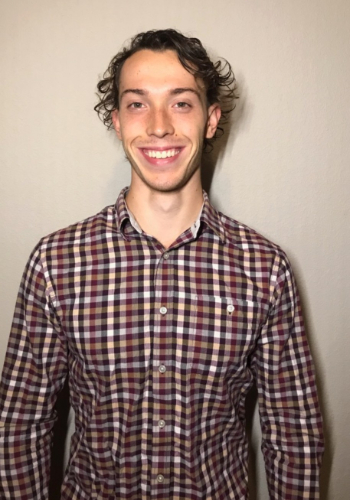
\includegraphics[width=\textwidth]{fmt-golba.jpg}
\end{minipage}
\begin{minipage}{0.73\textwidth}
$\textbf{Career Fair Coordinator - Grzegorz Golba}$\\
	Grzegorz Golba is a sophomore pursuing a B.S. in Nuclear Engineering with a physics minor in the plasma and fusion science concentration. He is now studying material interactions with plasma under Dr. Daniel Andruczyk. Grzegorz attended the 2019 ANS Student Conference in Virginia, reaffirmed his desire to study of nuclear science. He seeks new opportunities to engage with the nuclear science community and is excited for the possibilities of hosting a student conference at UIUC. 
\end{minipage}

\vspace{1cm}
\textbf{Non-Technical Subcommittee}\\

\begin{minipage}{0.25\textwidth}
	\centering
	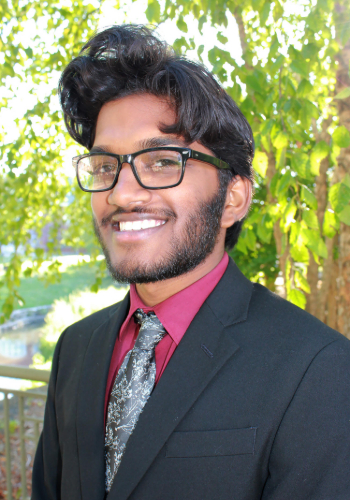
\includegraphics[width=\textwidth]{fmt-dilan.jpg}
\end{minipage}
\begin{minipage}{0.73\textwidth}
	$\textbf{Program Coordinator - Dilan Kurukulasuriya}$\\
Dilan Kurukulasuriay is a sophomore pursuing a B.S. in Nuclear, Plasma, and Radiological Engineering, along with a minor in Physics and Mathematics. He has been active in ANS at UIUC since the start of his freshman year, and he currently serves as the Outreach Chair on the Executive Board. Dilan has worked at the Center for Plasma-Material Interactions lab since the start of his freshman year on HIDRA, and he stayed on campus over the summer to continue to do so. Dilan attended the 2019 ANS Student Conference and it was the highlight of his freshman year of college. He is interested in fusion science research, specifically the materials interaction aspect. He also plans on attending the upcoming student conference at NC State in 2020.
\end{minipage}

\begin{minipage}{0.25\textwidth}
	\centering
	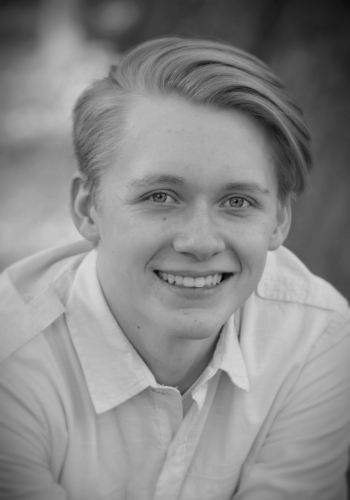
\includegraphics[width=\textwidth]{fmt-davis.jpg}
\end{minipage}
\begin{minipage}{0.73\textwidth}
$\textbf{Hotels and Transportation Coordinator - Gavin Davis}$\\
	Gavin is currently pursuing a B.S. in Nuclear, Plasma, and Radiological Engineering from UIUC and plans to graduate in 2022. He has been involved with the ANS-UIUC since his freshman year and has dedicated his time to outreach events and increasing public awareness of nuclear science and nuclear energy. He has accomplished this through events such as UIUC's Engineering Open House. It was an event he enjoyed as a kid and hopes to help other children develop an interest in nuclear sciences. He also returns to his high school to talk about his experience at UIUC. He looks forward to learning more about nuclear fission technology and to make advancements in nuclear science and in the nuclear energy sector as a whole. He looks forward to attending the student conference at NC State in 2020.
\end{minipage}

\begin{minipage}{0.25\textwidth}
	\centering
	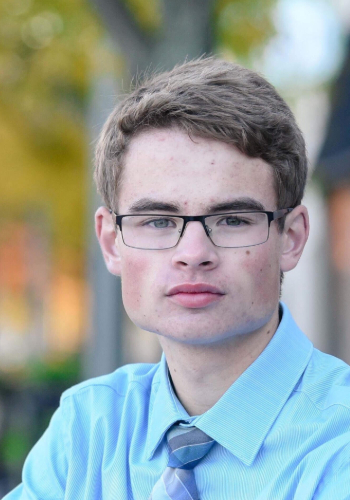
\includegraphics[width=\textwidth]{fmt-moran.jpg}
\end{minipage}
\begin{minipage}{0.73\textwidth}
	$\textbf{Hospitality and Catering Coordinator - Brady Moran}$\\
Brady a freshman in the Nuclear, Plasma, and Radiological Engineering program in the Plasma concentration. He is looking forward to putting his time and efforts toward ANS events throughout his years at UIUC. Last year, Brady planned a large tasting event, the Taste of Sauk Valley, which boasted 550 attendees, $\$$15,000 in revenue, and required him to coordinate 12 restaurants and various subcommittees. He is confident that this experience will help him make the Student Conference a great success. He will be attending the 2020 conference at NC State.
\end{minipage}

\begin{minipage}{0.25\textwidth}
	\centering
	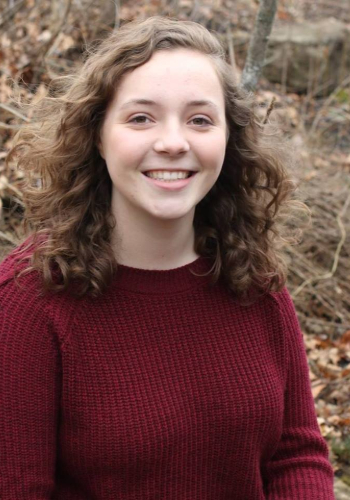
\includegraphics[width=\textwidth]{fmt-balla.jpg}
\end{minipage}
\begin{minipage}{0.73\textwidth}
	$\textbf{Tours Coordinator - Anna Balla}$\\
Anna is a junior in NPRE with a planned concentration in the power, safety, and the environment. She became interested in nuclear engineering after taking a general education class with an NPRE professor and learning about how effective nuclear power is at reducing carbon emissions. Anna is a teaching assistant for two classes in the NPRE department and is also very involved with the Women in Nuclear chapter at Illinois. In her spare time, she enjoys going to concerts, playing volleyball, and wishing she knew how to juggle.
\end{minipage}

\begin{minipage}{0.25\textwidth}
	\centering
	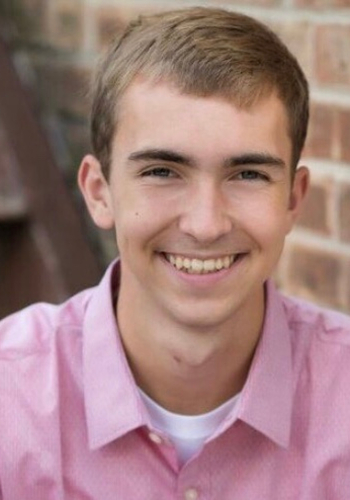
\includegraphics[width=\textwidth]{fmt-ryan.jpg}
\end{minipage}
\begin{minipage}{0.73\textwidth}
$\textbf{Media Coordinator - Nathan Ryan}$\\
	Nathan is pursuing a B.S. in Physics from UIUC. He graduated in the top five of his high school class, while holding down a part time managerial position and running a research project at Argonne National Laboratory concurrent with his Sophomore through Senior years of Secondary Education. His first experience with Nuclear Physics was at the National Superconducting Cyclotron Laboratory where he worked with grad students on rare Cadmium isotopes. He has experience with building appealing website pages, as well as social media communications. He believes that an online presence for this event will supplement the success of an already great set of programs and individuals involved. He is excited to attend the upcoming ANS Student Conference at NC State in 2020.
\end{minipage}

\subsection{Conflict Resolution}

Committee members should hold professionalism at the forefront of their composure in order to avoid and resolve issues amicably without the involvement of higher powers. As such, members are encouraged to settle conflicts without invoking this protocol. If an issue arises that immediately presents itself as overwhelming, the scope of the issue exceeds an individual’s ability to handle it, or the issue imposes certain implications that jeopardizes the mission of the planning committee, members should not hesitate to refer to this section. In the event of a conflict between members of the planning committee, a document for decision-making and
conflict resolution has been drafted and approved by the general committee. All General Committee members
are expected to abide by the resolution. Key points of the resolution are as follows:
\begin{enumerate}
	\item Subcommittees are encouraged to resolve conflicts internally and as democratically as possible. If an independent resolution cannot be reached, the Co-Chairs should be involved. The Co-Chairs have the final word on all decisions. If the Co-Chairs are unable to agree on a solution, the faculty advisor will be involved.
	\item Conflicts between individual committee members are to be resolved outside of the committee. Should such a conflict jeopradize the mission of the conference the Co-Chairs will be involved. 
	\item Any cases of misconduct or negligence will be handled appropriately by the Co-Chairs.
	\item For extreme cases of misconduct or negligence, separate steps for the removal and replacement of a
	member are outlined for general members, Subcommittee Chairs, and Co-Chairs. These include
	a discussion with the offending member, consultation of the Faculty Advisor, and a hearing with the
	General Committee to decide if removal is necessary.
\end{enumerate}

\subsection{Staffing Requirements}
Staffing for room breakdowns and setups, registration, socials, workshops, 
tours, etc.  will be supplied by either UIUC ANS members or students of the 
NPRE department. While it is likely that members of our student chapter will 
voluntarily fill all the staffing requirements of conference hosted events. If 
not, we will rely on other student organizations for support including, but not 
limited to: Arms Control and Domestic and International Security (ACDIS) and 
Women in Engineering (WIE). Participating in conference events on a staff level 
is a beneficial experience for any undergraduate who wants to become more 
familiar with ANS or support their ANS Chapter. Throughout the conference, 
interacting with registering students, driving groups to tour a scientific 
facility, and turning rooms for technical sessions provide plentiful 
opportunities for volunteers to interact with myriad members on a number of 
levels. Thus, it will be an overall positive experience for the volunteers. 
Quantitative needs are outlined in Appendix \ref{appendix:staff} on page 
\pageref{appendix:staff}.

% ===============================================
% Milestones
% ===============================================
\newpage
\subsection{Milestones}

\begin{center}
\begin{longtable}{c |  c  c}
\hline\hline
\textbf{Deadline} & \textbf{Task} & \textbf{Responsible Committee}\\
\hline\hline

&\textbf{November}&\\
\hline\hline
11/21/19 & Announcement of 2021 Conference & \\
11/21/19 & Update milestones with lessons learned &\\
11/21/19 & Notify department of selection & Co-Chairs\\
11/22/19 & Confirm Conference Committee & Co-Chairs\\
11/29/19 & Finalize Conference Date & Co-Chairs\\
\hline\hline
&\textbf{December}&\\
\hline\hline
12/1/19 & Contact ANS National for support with hotel negotiations& Co-Chairs and Non-Technical\\
12/1/19 & Set up banking through Busey Bank and ANS National& Financial\\
12/3/19 & Confirm Conference Reservations & Non-Technical\\
12/3/19 & Finalize Facilities Reservations& Non-Technical\\
12/20/19 & Finalize Logo Design& Media\\
12/20/19 & Begin Designing Website and Social Media& Media\\
\hline\hline
&$\textbf{2020}$&\\
\hline\hline
&\textbf{January}&\\
\hline\hline
1/13/20 & Finalize meeting schedule& Co-Chairs\\
\hline\hline
&\textbf{February}&\\
\hline\hline
2/3/20 & Launch social media plan& Media\\
2/17/20 & Finalize list of potential speakers& Non-Technical\\
2/17/20 & Finalize technical topics& Technical\\
\hline\hline
&\textbf{March}&\\
\hline\hline
3/9/20 & Contact Speakers and Presenters& Non-Technical and Technical\\
3/26-28/20 & Attend Student Conference at NC State& All\\
3/28/20 & Request lessons learned from NC State& Co-Chairs\\
\hline\hline
&\textbf{April}&\\
\hline\hline
4/6/20 & Create sponsor letters and contact & General Co-Chair\\
4/13/20 & Prepare tour opportunities& Non-Technical\\
\hline\hline
&\textbf{May}&\\
\hline\hline
5/4/20 & Confirm tours and costs& Non-Technical\\
5/18/20 & Submit Progress Report to SSC& Co-Chairs\\
5/18/20 & Create a Call for Papers & Technical and Media\\
\hline\hline
&\textbf{June}&\\
\hline\hline
6/7-11/20 & Send Delegates to Annual Meeting in Arizona& Co-Chairs, All\\
\hline\hline
&\textbf{July}&\\
\hline\hline
7/6/20 & Confirm with all speakers and presenters& Technical\\
7/20/20 & Report on sponsorship& Financial\\
7/27/20 & Reassess budget& Financial\\
\hline\hline
&\textbf{August}&\\
\hline\hline
8/10/20 & Update with sponsors& Financial\\
8/24/20 & Submit second progress to SSC& Co-Chairs\\
\hline\hline
&\textbf{September}&\\
\hline\hline
9/14/20 & Updates on conference deadlines& Financial\\
9/21/20 & Finalize gift bag order& Non-Technical\\
\hline\hline
&\textbf{October}&\\
\hline\hline
10/12/20 & Confirm hotel blocks and contracts& Non-Technical\\
10/26/20 & Registration Opens& Financial\\
10/26/20 & Create and test online paper submission& Technical\\
\hline\hline
&\textbf{November}&\\
\hline\hline
11/15-19/20 & Attend Winter Conference 2020 in Chicago& Co-Chairs, All\\
11/24/20 & Finalize marketing material& Media\\
11/24/20 & Report from winter conference & Co-Chairs\\
\hline\hline
&\textbf{December}&\\
\hline\hline
12/4/20 & Reassess Budget & Financial \\
12/4/20 & Update website & Media \\
12/18/20 & Third progress report to SSC& Co-Chairs\\
12/18/20 & Send out call for papers& Media\\
\hline\hline
&$\textbf{2021}$&\\
\hline\hline
&\textbf{January}&\\
\hline\hline
1/4/20 & Confirm all judges, panelists, and speakers& Technical\\
1/18/20 & First paper deadline -- send to reviewers & Technical\\
1/22/20 & Recruit student volunteers& All\\
1/29/21 & Finalize tours& Non-Technical\\
1/29/21& Finalize conference transportation& Non-Technical\\
\hline\hline
&\textbf{February}&\\
\hline\hline
2/1/21 & Finalize program& Media\\
2/1/21 & Order gift bag items & Financial and Non-Technical\\
2/5/21 & Final Paper Deadline& Technical\\
2/9/21 & Extended Paper Deadline& \\
2/15/21 & Finalize Website& Media\\
2/19/21 & Finalize budget& Financial\\
\hline\hline
&\textbf{March}&\\
\hline\hline
3/22/21 & Print Programs& Media\\
3/26/21 & Finalize Awards& Technical\\
3/26/21 & Finalize Staff Schedule& Non-Technical\\
3/29/21 & Final progress report to SSC& Co-Chairs\\
\hline\hline
&\textbf{April}&\\
\hline\hline
4/1/21 & Prepare gift bags, print tags, and banners& Non-Technical\\
4/8-11/21 & Host ANS Student Conference 2021 & \\
4/22/21 & Return seed money& Financial\\
4/29/21 & Process Student Reimbursements& Financial\\
4/29/21 & Finalize financial report& Financial\\
4/29/21 & Submit conference report& Co-Chairs\\
\hline\hline
\end{longtable}
\end{center}
